\documentclass[border=10pt]{standalone}
\usepackage{tikz}
\usetikzlibrary{arrows.meta, shapes.geometric, calc, decorations.pathreplacing, positioning, fit}

\begin{document}
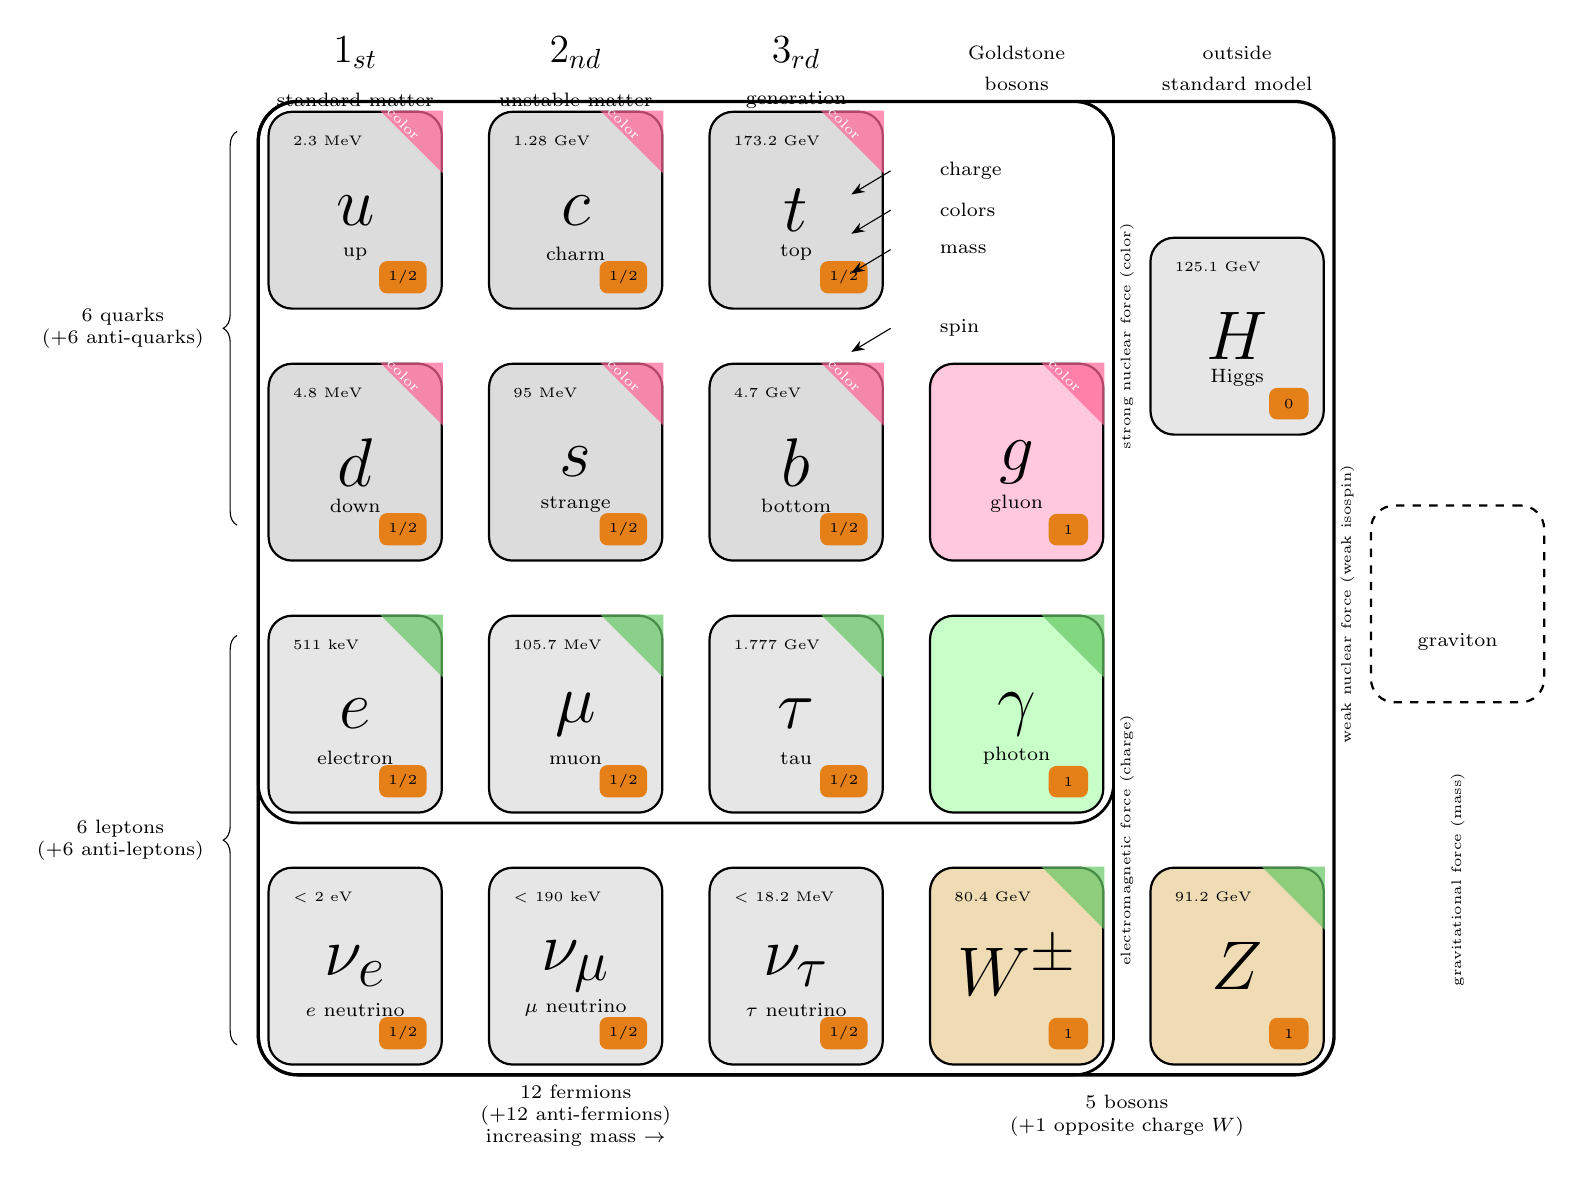
\begin{tikzpicture}[
    particle/.style={
        rectangle, rounded corners=3mm, minimum width=2.2cm, minimum height=2.5cm,
        draw=black, line width=0.8pt, fill=#1
    },
    ribbon/.style={
        fill=#1, opacity=0.7
    },
    spin/.style={
        rectangle, rounded corners=1mm, fill=orange!60!brown, minimum width=0.5cm, minimum height=0.4cm
    }
]

% Define colors
\definecolor{quarkbg}{RGB}{220,220,220}
\definecolor{leptonbg}{RGB}{230,230,230}
\definecolor{gluonbg}{RGB}{255,200,220}
\definecolor{photonbg}{RGB}{200,255,200}
\definecolor{bosonbg}{RGB}{240,220,180}
\definecolor{higgsbg}{RGB}{230,230,230}
\definecolor{ribbonpink}{RGB}{255,100,150}
\definecolor{ribbongreen}{RGB}{100,200,100}

% Quarks - First generation
\node[particle=quarkbg] (u) at (0,0) {};
\node at (u.north west) [anchor=north west, xshift=2mm, yshift=-2mm, font=\tiny] {2.3 MeV};
\node at (u.center) [font=\Huge\itshape] {$u$};
\node at (u.south) [anchor=south, yshift=5mm, font=\scriptsize] {up};
\node[spin] at (u.south east) [anchor=south east, xshift=-2mm, yshift=2mm] {\tiny $1/2$};
\fill[ribbonpink, opacity=0.7] (u.north east) -- ++(-0.8,0) -- ++(0.8,-0.8) -- cycle;
\node at (u.north east) [anchor=north east, xshift=-1mm, yshift=-3mm, font=\tiny, rotate=-45, text=white] {color};

\node[particle=quarkbg] (d) at (0,-3.2) {};
\node at (d.north west) [anchor=north west, xshift=2mm, yshift=-2mm, font=\tiny] {4.8 MeV};
\node at (d.center) [font=\Huge\itshape] {$d$};
\node at (d.south) [anchor=south, yshift=5mm, font=\scriptsize] {down};
\node[spin] at (d.south east) [anchor=south east, xshift=-2mm, yshift=2mm] {\tiny $1/2$};
\fill[ribbonpink, opacity=0.7] (d.north east) -- ++(-0.8,0) -- ++(0.8,-0.8) -- cycle;
\node at (d.north east) [anchor=north east, xshift=-1mm, yshift=-3mm, font=\tiny, rotate=-45, text=white] {color};

% Quarks - Second generation
\node[particle=quarkbg] (c) at (2.8,0) {};
\node at (c.north west) [anchor=north west, xshift=2mm, yshift=-2mm, font=\tiny] {1.28 GeV};
\node at (c.center) [font=\Huge\itshape] {$c$};
\node at (c.south) [anchor=south, yshift=5mm, font=\scriptsize] {charm};
\node[spin] at (c.south east) [anchor=south east, xshift=-2mm, yshift=2mm] {\tiny $1/2$};
\fill[ribbonpink, opacity=0.7] (c.north east) -- ++(-0.8,0) -- ++(0.8,-0.8) -- cycle;
\node at (c.north east) [anchor=north east, xshift=-1mm, yshift=-3mm, font=\tiny, rotate=-45, text=white] {color};

\node[particle=quarkbg] (s) at (2.8,-3.2) {};
\node at (s.north west) [anchor=north west, xshift=2mm, yshift=-2mm, font=\tiny] {95 MeV};
\node at (s.center) [font=\Huge\itshape] {$s$};
\node at (s.south) [anchor=south, yshift=5mm, font=\scriptsize] {strange};
\node[spin] at (s.south east) [anchor=south east, xshift=-2mm, yshift=2mm] {\tiny $1/2$};
\fill[ribbonpink, opacity=0.7] (s.north east) -- ++(-0.8,0) -- ++(0.8,-0.8) -- cycle;
\node at (s.north east) [anchor=north east, xshift=-1mm, yshift=-3mm, font=\tiny, rotate=-45, text=white] {color};

% Quarks - Third generation
\node[particle=quarkbg] (t) at (5.6,0) {};
\node at (t.north west) [anchor=north west, xshift=2mm, yshift=-2mm, font=\tiny] {173.2 GeV};
\node at (t.center) [font=\Huge\itshape] {$t$};
\node at (t.south) [anchor=south, yshift=5mm, font=\scriptsize] {top};
\node[spin] at (t.south east) [anchor=south east, xshift=-2mm, yshift=2mm] {\tiny $1/2$};
\fill[ribbonpink, opacity=0.7] (t.north east) -- ++(-0.8,0) -- ++(0.8,-0.8) -- cycle;
\node at (t.north east) [anchor=north east, xshift=-1mm, yshift=-3mm, font=\tiny, rotate=-45, text=white] {color};

\node[particle=quarkbg] (b) at (5.6,-3.2) {};
\node at (b.north west) [anchor=north west, xshift=2mm, yshift=-2mm, font=\tiny] {4.7 GeV};
\node at (b.center) [font=\Huge\itshape] {$b$};
\node at (b.south) [anchor=south, yshift=5mm, font=\scriptsize] {bottom};
\node[spin] at (b.south east) [anchor=south east, xshift=-2mm, yshift=2mm] {\tiny $1/2$};
\fill[ribbonpink, opacity=0.7] (b.north east) -- ++(-0.8,0) -- ++(0.8,-0.8) -- cycle;
\node at (b.north east) [anchor=north east, xshift=-1mm, yshift=-3mm, font=\tiny, rotate=-45, text=white] {color};

% Leptons - First generation
\node[particle=leptonbg] (e) at (0,-6.4) {};
\node at (e.north west) [anchor=north west, xshift=2mm, yshift=-2mm, font=\tiny] {511 keV};
\node at (e.center) [font=\Huge\itshape] {$e$};
\node at (e.south) [anchor=south, yshift=5mm, font=\scriptsize] {electron};
\node[spin] at (e.south east) [anchor=south east, xshift=-2mm, yshift=2mm] {\tiny $1/2$};
\fill[ribbongreen, opacity=0.7] (e.north east) -- ++(-0.8,0) -- ++(0.8,-0.8) -- cycle;

\node[particle=leptonbg] (nue) at (0,-9.6) {};
\node at (nue.north west) [anchor=north west, xshift=2mm, yshift=-2mm, font=\tiny] {$<$ 2 eV};
\node at (nue.center) [font=\Huge\itshape] {$\nu_e$};
\node at (nue.south) [anchor=south, yshift=5mm, font=\scriptsize] {$e$ neutrino};
\node[spin] at (nue.south east) [anchor=south east, xshift=-2mm, yshift=2mm] {\tiny $1/2$};

% Leptons - Second generation
\node[particle=leptonbg] (mu) at (2.8,-6.4) {};
\node at (mu.north west) [anchor=north west, xshift=2mm, yshift=-2mm, font=\tiny] {105.7 MeV};
\node at (mu.center) [font=\Huge\itshape] {$\mu$};
\node at (mu.south) [anchor=south, yshift=5mm, font=\scriptsize] {muon};
\node[spin] at (mu.south east) [anchor=south east, xshift=-2mm, yshift=2mm] {\tiny $1/2$};
\fill[ribbongreen, opacity=0.7] (mu.north east) -- ++(-0.8,0) -- ++(0.8,-0.8) -- cycle;

\node[particle=leptonbg] (numu) at (2.8,-9.6) {};
\node at (numu.north west) [anchor=north west, xshift=2mm, yshift=-2mm, font=\tiny] {$<$ 190 keV};
\node at (numu.center) [font=\Huge\itshape] {$\nu_\mu$};
\node at (numu.south) [anchor=south, yshift=5mm, font=\scriptsize] {$\mu$ neutrino};
\node[spin] at (numu.south east) [anchor=south east, xshift=-2mm, yshift=2mm] {\tiny $1/2$};

% Leptons - Third generation
\node[particle=leptonbg] (tau) at (5.6,-6.4) {};
\node at (tau.north west) [anchor=north west, xshift=2mm, yshift=-2mm, font=\tiny] {1.777 GeV};
\node at (tau.center) [font=\Huge\itshape] {$\tau$};
\node at (tau.south) [anchor=south, yshift=5mm, font=\scriptsize] {tau};
\node[spin] at (tau.south east) [anchor=south east, xshift=-2mm, yshift=2mm] {\tiny $1/2$};
\fill[ribbongreen, opacity=0.7] (tau.north east) -- ++(-0.8,0) -- ++(0.8,-0.8) -- cycle;

\node[particle=leptonbg] (nutau) at (5.6,-9.6) {};
\node at (nutau.north west) [anchor=north west, xshift=2mm, yshift=-2mm, font=\tiny] {$<$ 18.2 MeV};
\node at (nutau.center) [font=\Huge\itshape] {$\nu_\tau$};
\node at (nutau.south) [anchor=south, yshift=5mm, font=\scriptsize] {$\tau$ neutrino};
\node[spin] at (nutau.south east) [anchor=south east, xshift=-2mm, yshift=2mm] {\tiny $1/2$};

% Bosons
\node[particle=gluonbg] (g) at (8.4,-3.2) {};
\node at (g.center) [font=\Huge\itshape] {$g$};
\node at (g.south) [anchor=south, yshift=5mm, font=\scriptsize] {gluon};
\node[spin] at (g.south east) [anchor=south east, xshift=-2mm, yshift=2mm] {\tiny $1$};
\fill[ribbonpink, opacity=0.7] (g.north east) -- ++(-0.8,0) -- ++(0.8,-0.8) -- cycle;
\node at (g.north east) [anchor=north east, xshift=-1mm, yshift=-3mm, font=\tiny, rotate=-45, text=white] {color};

\node[particle=photonbg] (gamma) at (8.4,-6.4) {};
\node at (gamma.center) [font=\Huge\itshape] {$\gamma$};
\node at (gamma.south) [anchor=south, yshift=5mm, font=\scriptsize] {photon};
\node[spin] at (gamma.south east) [anchor=south east, xshift=-2mm, yshift=2mm] {\tiny $1$};
\fill[ribbongreen, opacity=0.7] (gamma.north east) -- ++(-0.8,0) -- ++(0.8,-0.8) -- cycle;

\node[particle=bosonbg] (W) at (8.4,-9.6) {};
\node at (W.north west) [anchor=north west, xshift=2mm, yshift=-2mm, font=\tiny] {80.4 GeV};
\node at (W.center) [font=\Huge\itshape] {$W^\pm$};
\node[spin] at (W.south east) [anchor=south east, xshift=-2mm, yshift=2mm] {\tiny $1$};
\fill[ribbongreen, opacity=0.7] (W.north east) -- ++(-0.8,0) -- ++(0.8,-0.8) -- cycle;

\node[particle=bosonbg] (Z) at (11.2,-9.6) {};
\node at (Z.north west) [anchor=north west, xshift=2mm, yshift=-2mm, font=\tiny] {91.2 GeV};
\node at (Z.center) [font=\Huge\itshape] {$Z$};
\node[spin] at (Z.south east) [anchor=south east, xshift=-2mm, yshift=2mm] {\tiny $1$};
\fill[ribbongreen, opacity=0.7] (Z.north east) -- ++(-0.8,0) -- ++(0.8,-0.8) -- cycle;

% Higgs
\node[particle=higgsbg] (H) at (11.2,-1.6) {};
\node at (H.north west) [anchor=north west, xshift=2mm, yshift=-2mm, font=\tiny] {125.1 GeV};
\node at (H.center) [font=\Huge\itshape] {$H$};
\node at (H.south) [anchor=south, yshift=5mm, font=\scriptsize] {Higgs};
\node[spin] at (H.south east) [anchor=south east, xshift=-2mm, yshift=2mm] {\tiny $0$};

% Graviton (dashed box)
\node[particle=white, dashed] (graviton) at (14,-5) {
    \begin{tabular}{c}
        \\[5mm]
        {\scriptsize graviton}
    \end{tabular}
};

% Boxes and labels
% Inner box for quarks and leptons
\node[draw, rounded corners=5mm, line width=1pt, fit=(u)(d)(c)(s)(t)(b)(g)(gamma)] (fermionbox) {};

% Box for all fermions including neutrinos
\node[draw, rounded corners=5mm, line width=1pt, fit=(u)(d)(c)(s)(t)(b)(e)(mu)(tau)(nue)(numu)(nutau)(g)(gamma)] (allbox) {};

% Outer box for standard model
\node[draw, rounded corners=5mm, line width=1.2pt, fit=(u)(d)(c)(s)(t)(b)(e)(mu)(tau)(nue)(numu)(nutau)(g)(gamma)(W)(Z)(H)] (smbox) {};

% Labels at top
\node at (0,2) [font=\Large] {$1_{\text{st}}$};
\node at (0,1.4) [font=\scriptsize] {standard matter};

\node at (2.8,2) [font=\Large] {$2_{\text{nd}}$};
\node at (2.8,1.4) [font=\scriptsize] {unstable matter};

\node at (5.6,2) [font=\Large] {$3_{\text{rd}}$};
\node at (5.6,1.4) [font=\scriptsize] {generation};

\node at (8.4,2) [font=\scriptsize] {Goldstone};
\node at (8.4,1.6) [font=\scriptsize] {bosons};

\node at (11.2,2) [font=\scriptsize] {outside};
\node at (11.2,1.6) [font=\scriptsize] {standard model};

% Arrows and labels for particle properties
\draw[-Stealth] (6.8,0.5) -- (6.3,0.2);
\node at (7.3,0.5) [anchor=west, font=\scriptsize] {charge};

\draw[-Stealth] (6.8,0) -- (6.3,-0.3);
\node at (7.3,0) [anchor=west, font=\scriptsize] {colors};

\draw[-Stealth] (6.8,-0.5) -- (6.3,-0.8);
\node at (7.3,-0.5) [anchor=west, font=\scriptsize] {mass};

\draw[-Stealth] (6.8,-1.5) -- (6.3,-1.8);
\node at (7.3,-1.5) [anchor=west, font=\scriptsize] {spin};

% Left side labels
\draw[decorate, decoration={brace, amplitude=5pt, mirror}] (-1.5,1) -- (-1.5,-4) 
    node[midway, left, xshift=-3mm, align=center, font=\scriptsize] {6 quarks\\(+6 anti-quarks)};

\draw[decorate, decoration={brace, amplitude=5pt, mirror}] (-1.5,-5.4) -- (-1.5,-10.6) 
    node[midway, left, xshift=-3mm, align=center, font=\scriptsize] {6 leptons\\(+6 anti-leptons)};

% Bottom labels
\node at (2.8,-11.5) [font=\scriptsize, align=center] {12 fermions\\(+12 anti-fermions)\\increasing mass $\rightarrow$};

\node at (9.8,-11.5) [font=\scriptsize, align=center] {5 bosons\\(+1 opposite charge $W$)};

% Vertical text labels
\node at (9.8,-1.6) [font=\tiny, rotate=90] {strong nuclear force (color)};
\node at (9.8,-8) [font=\tiny, rotate=90] {electromagnetic force (charge)};
\node at (12.6,-5) [font=\tiny, rotate=90] {weak nuclear force (weak isospin)};
\node at (14,-8.5) [font=\tiny, rotate=90] {gravitational force (mass)};

\end{tikzpicture}
\end{document}